
% Basic template for homeworks
% derived from miktex's article template
% Roger Fowler
% 30 September 2024

\documentclass[10pt]{article} % set font size
\usepackage[utf8]{inputenc} % set input encoding (not needed with XeLaTeX)

\usepackage{geometry} % to change the page dimensions
\geometry{a4paper}

\usepackage{graphicx} % support the \includegraphics command and options
\usepackage{booktabs} % for much better looking tables
\usepackage{array} % for better arrays (eg matrices) in maths
\usepackage{paralist} % very flexible & customisable lists (eg. enumerate/itemize, etc.)
\usepackage{verbatim} % adds environment for commenting out blocks of text & for better verbatim
\usepackage{subfig} % make it possible to include more than one captioned figure/table in a single float
\usepackage{mathtools} % get split environment
\usepackage{amsmath}
\usepackage{cancel} % get /cancel command
\usepackage{tikz} % for drawing geometry
\usepackage{tkz-euclide} % specifically for calculating intersections
\usepackage{amssymb} % get \triangleq
\usepackage{matlab-prettifier} % for including matlab code in a \begin{lstlisting}[style=Matlab-editor] block

\usepackage{fancyhdr} % headers and footers
\pagestyle{plain} % options: empty , plain , fancy

\usepackage{sectsty} % section titles
\renewcommand\thesection{\arabic{section}} % sections are numbered
\renewcommand\thesubsection{\thesection)\alph{subsection}} % subsections are lettered
% options are:
%    \arabic (1, 2, 3, ...)
%    \alph (a, b, c, ...)
%    \Alph (A, B, C, ...)
%    \roman (i, ii, iii, ...)
%    \Roman (I, II, III, ...)
%    \fnsymbol (∗, †, ‡, §, ¶, ...)
%

%\allsectionsfont{\sffamily\mdseries\upshape} % (See the fntguide.pdf for font help)
\usepackage{titlesec}
\titleformat{\section}[hang]
{\normalfont\bfseries}
{\thesection}{0.5em}{}
\titleformat{\subsection}[hang]
{\normalfont\bfseries}
{\thesubsection}{0.5em}{}
\titleformat{\subsubsection}[hang]
{\normalfont\bfseries}
{\thesubsubsection}{0.5em}{}

\renewcommand\deg{^\circ} % define degree symbol as \deg

% matrix display commands
\newcommand{\skewmat}[3]{\begin{bmatrix}0&-#3&#2\\#3&0&-#1\\-#2&#1&0\end{bmatrix}}
\newcommand{\diagmat}[3]{\begin{bmatrix}#1&0&0\\0&#2&0\\0&0&#3\end{bmatrix}}
\newcommand{\vecmat}[3]{\begin{bmatrix}#1\\#2\\#3\end{bmatrix}}

% laplace transform commands
\newcommand{\Lapl}[1]{\mathcal{L}\left\{#1\right\}}
\newcommand{\invLapl}[1]{\mathcal{L}^{-1}\left\{#1\right\}}

% rotated text
\usepackage{rotating}

% table stuff
\usepackage{multirow}

% pseudocode formatting
\usepackage{algorithm}
\usepackage{algpseudocode}

% enumerate compression
\usepackage{enumitem}

%%% END Article customizations

\title{\vspace{-2cm}Multi-Agent Training in the Wizard Card Game\\{\large CS 5180 - Reinforcement Learning and Sequential Decision Making}}
\author{Roger Fowler}
\date{April 18 2025}

\begin{document}
\maketitle

\section{Problem Statement}

Wizard is a trick-taking card game for three to six players. Each hand is composed of a number of tricks. After being dealt hands, players must bet exactly how many tricks they will win during the play of the hand. Rules during play may make cards more or less valuable: the current trump suit is the most valuable, followed by the suit led by the first player of that trick. Players also must follow the led suit if possible. Whichever player wins the trick leads the next suit. In addition to the normal 52 card deck, there are also 4 Wizard cards which will beat anything except a previous Wizard, and 4 Jester cards which will not beat anything except a following Jester. Pseudocode for playing a game is detailed in the appendix in Algorithm \ref{alg:game}.

The rules of the game are such that a player only receives points if they win exactly their bet number of tricks; otherwise they lose points. The game has no house to compete against and no stochastic transitions after dealing; only the randomness of the deck and the decisions of the players affect the state. It is also a non-zero sum game that requires balancing cooperation and competition. For these reasons, the game is complex enough to justify a machine learning effort beyond a toy problem. On a technical level there are a few challenges: state transitions and rewards are stochastic for an agent because other agents cannot be predicted, agents have only partial knowledge of game state, the changing led suit alters the values of cards from trick to trick, and agents can be forced to take actions to follow the led suit.

\section{Development}

Development was initially planned for the python Gymnasium environment, which has poor support for multi-agent training, then transitioned to the PettingZoo environment, but this is not well-maintained, so a custom python environment was implemented without library support. The custom environment must keep track of game state. At each turn it is queried for the current agent, then it must produce a state observation and action mask for that agent. The agent is queried for its action, which is fed back to the environment, and receives a reward.

Due to the number of possible states, with $60!$ deck shufflings permuted by up to $60$ consecutive player actions, agents were required to be neural networks. Agents were implemented in a modular manner to allow for ease of use. Each agent is dynamically constructed from a json file containing: a neural net architecture, an epsilon schedule, a buffer priority function, and other parameters. Pytorch was used to construct and train all neural nets. Some parameters were kept constant across all trials to reduce the possible combinations (Table \ref{tab:params}). Agents were trained by performing $\varepsilon$-greedy actions, sampling from a buffer of previous actions, and optimizing a neural net to minimize loss of estimated future returns $Q(s,a)$ with respect to a constant target neural net. Discounting is not applied to rewards since hands are of a set length with all points awarded at the end.

\begin{table}[h!]
\centering
\begin{tabular}{r|l}
Number of Players & 4 \\
Training Timesteps & $500,000$ \\
Replay Buffer Size & $50,000$ \\
\multirow{2}{*}{
Behavior Network Update
$\left\{\begin{matrix}
\text{Period} \\ \text{Batch Size}
\end{matrix}\right.$}
& 4 \\
& 32 \\
Target Network Update Period & 2000 \\
\multirow{2}{*}{
Optimizer
$\left\{\begin{matrix}
\text{Type} \\ \text{Learning Rate}
\end{matrix}\right.$}
& Adam \\
& 0.001 \\
\multirow{4}{*}{
Epsilon Schedule
$\left\{\begin{matrix}
\text{Type} \\ \text{Max} \\ \text{Min} \\ \text{Duration}
\end{matrix}\right.$}
& Linear \\
& 1 \\
& 0.01 \\
& $250,000$ \\
Loss & Mean Squared Error \\
\end{tabular}
\caption{Standard Training Parameters} \label{tab:params}
\end{table}

\newpage

\subsection{State Representation}

The environment provides to each agent several pieces of information:

\setlist{nolistsep}
\begin{enumerate}[noitemsep]
\item Cards in their hand
\item Trump suit
\item Led suit
\item Cards which have been played
\item Who led the hand
\item Bet amount
\item Tricks won
\item Tricks remaining
\end{enumerate}

Some of these are redundant: who led the trick is obvious by the number of cards in the current pile; the led suit is the suit of the first card in the pile, and is not defined if there is no pile. Tricks remaining is equal to the number of cards in hand. Bet amount and tricks won can be combined into the number of tricks that must still be won to make the bet. In this case the agent can only decrease this number and will aim for zero. But decreasing it past zero will incur a penalty at scoring time.

The 60 card deck is distributed among several groups; with some number of known cards in hand, a known card flipped to reveal trump suit, known cards that have been played, and the rest of the unknown cards distributed between the remaining undealt deck and the other agents’ hands. In fact, there is additional information here; an agent may not know which specific cards are in another agent’s hand, but because an agent can be forced to play the led suit, if they do not do so implies that they have no cards of that suit. However, this last bit is difficult to represent and will be ignored.

Suits are fungible, except that one or zero is the trump suit for the hand and one or zero, possibly the same as trump, is the led suit for the trick. The deck can be sorted to place cards in order of value: wizards first, then trump suit from high to low, then led suit, then the other two suits in a consistent order, then jesters. Padding the deck to always be the same size allows for more consistent evaluation. Also, placing like-valued cards together may allow the deck to have local features which can be convolved.

The final state is therefore a 65 element vector (Table \ref{tab:state}).

\begin{table}[h!]
\centering
\begin{tabular}{r|c|l}
Index & Value & Description \\ \hline
0 & $bet - won$ & how many tricks the agent needs to win \\
1 & $\sum bet - \sum won$ & how many tricks need to be won across all agents \\
2 & $N$ & number of players \\
3 & [0,1] & whether there is a trump suit \\
4 & [0,1] & whether the led suit is also the trump suit \\
5-64 &
$\begin{cases}
2 & \text{in pile} \\
1 & \text{in hand} \\
0 & \text{unseen} \\
-1 & \text{in previous piles} \\
\end{cases}$
& padded and sorted deck state
\end{tabular}
\caption{State Vector Definition} \label{tab:state}
\end{table}

State transitions become simplified in this representation. A state is composed of a hand of N cards and a goal of T remaining tricks to win. After an action is taken, the rest of the agents take their actions, and the agent arrives at a new state. This state will have exactly N-1 cards, and the agent is in control of which card was removed. However, it is generally not in control of whether T has remained the same or decreased by exactly one. Eventually this leads to a state where there are no cards in hand. In these states, any action (which can be restricted to a single null action) gives a reward and leads to a final terminal state. This reward is only positive when the bet was achieved (T=0) and increasingly negative otherwise. Also, since the agent has no control over the length of the game it does not make sense to discount rewards.

\subsection{Action Definitions}

The action space is large, but the permissible actions in any given state are small. An agent may bet from $[0-M]$ in trick $M$. During play an agent may play any legal card in its hand. Action masks are generated by the environment.

\begin{table}[h!]
\centering
\begin{tabular}{|c|c|} \hline
Index & Action \\ \hline
[0, 59] & play card with index $i$ \\ \hline
[60, 80] & bet $i-60$ \\ \hline
[81, 84] & choose trump suit \\ \hline
[85] & receive reward \\ \hline
\end{tabular}
\caption{Action Space Definition} \label{tab:actions}
\end{table}

\subsection{State Transitions}

Normal state transitions are simple; the chosen bet is stored or the chosen card is added to the pile. However, at the end of a trick an agent must be declared a winner. Starting with the trick leader we proceed around the table comparing cards. If a card is better than the current winner, that card becomes the winner. The possibilities are encoded in Table \ref{tab:trickwinner}.

\begin{table}
\centering
\addtolength{\leftskip}{-2cm}
\addtolength{\rightskip}{-2cm}
\begin{tabular}{ccc}
\begin{tabular}{c|l}
\multicolumn{2}{c}{Legend} \\ \hline
Y & New Card Wins \\
X & Current Winner Remains \\
$>$ & Compare Card Values \\
N/A & Impossible \\
\end{tabular}
& \hspace{5mm} &
\begin{tabular}{rrccccc}
\multicolumn{1}{l}{}      & \multicolumn{1}{l}{}        & \multicolumn{5}{c}{Current Winner}                                                                                                                                               \\
\multicolumn{1}{l}{}      & \multicolumn{1}{l}{}        & Wizard                              & Trump                               & Led                                 & Other                    & Jester                              \\ \cline{3-7} 
\multirow{5}{*}{\begin{turn}{90}New Card\end{turn}} & \multicolumn{1}{r|}{Wizard} & \multicolumn{1}{c|}{\textgreater{}} & \multicolumn{1}{c|}{\textgreater{}} & \multicolumn{1}{c|}{\textgreater{}} & \multicolumn{1}{c|}{N/A} & \multicolumn{1}{c|}{\textgreater{}} \\ \cline{3-7} 
                          & \multicolumn{1}{r|}{Trump}  & \multicolumn{1}{c|}{\textgreater{}} & \multicolumn{1}{c|}{\textgreater{}} & \multicolumn{1}{c|}{Y}              & \multicolumn{1}{c|}{N/A} & \multicolumn{1}{c|}{\textgreater{}} \\ \cline{3-7} 
                          & \multicolumn{1}{r|}{Led}    & \multicolumn{1}{c|}{\textgreater{}} & \multicolumn{1}{c|}{X}              & \multicolumn{1}{c|}{\textgreater{}} & \multicolumn{1}{c|}{N/A} & \multicolumn{1}{c|}{\textgreater{}} \\ \cline{3-7} 
                          & \multicolumn{1}{r|}{Other}  & \multicolumn{1}{c|}{\textgreater{}} & \multicolumn{1}{c|}{X}              & \multicolumn{1}{c|}{X}              & \multicolumn{1}{c|}{N/A} & \multicolumn{1}{c|}{\textgreater{}} \\ \cline{3-7} 
                          & \multicolumn{1}{r|}{Jester} & \multicolumn{1}{c|}{\textgreater{}} & \multicolumn{1}{c|}{\textgreater{}} & \multicolumn{1}{c|}{\textgreater{}} & \multicolumn{1}{c|}{N/A} & \multicolumn{1}{c|}{\textgreater{}} \\ \cline{3-7} 
\end{tabular}
\end{tabular}
\caption{Trick Winner Logic}
\label{tab:trickwinner}
\end{table}

\newpage

\section{Neural Network Structure}

The final neural network structure (Figure \ref{fig:network}) was determined iteratively. The state header, composed of dissimilar values, is fed through fully connected layers. The deck state, which should have local structure, is fed through convolutional layers. The combined state is then fed through a dueling network to account for the large number of actions. State value evaluation is given fewer neurons than action advantage. Action value is evaluated as:

\begin{equation}
Q(s,a) = V(s) + A(s,a) - \sum_a A(s,a)
\end{equation}

Agents were also pooled together; all players in a game shared a data buffer and a neural network but took actions based on their distinct observations.

\tikzstyle{round} = [rectangle, rounded corners, 
minimum width=1cm, 
minimum height=1cm,
text centered, 
draw=black, 
fill=cyan!30]

\tikzstyle{rect} = [rectangle, 
minimum width=1cm, 
minimum height=1cm, 
text centered,  
draw=black, 
fill=orange!30]

\tikzstyle{arrow} = [thick,->,>=stealth]

\begin{figure}[h!]
\centering
\addtolength{\leftskip}{-2cm}
\addtolength{\rightskip}{-2cm}
\begin{tikzpicture}[node distance=3cm]

\node(header) [rect] {Header};
\node(deck) [rect, below of=header, minimum height=4cm] {Deck};

\node(fullIn) [round, right of=header] {$\begin{matrix}\text{Fully Connected}\\\text{Layers: 2}\\\text{Width: 16}\end{matrix}$};
\node(convIn) [round, below of=fullIn, minimum height=4cm] {$\begin{matrix}\text{Convolutional}\\\text{Layers: 2}\\\text{Kernel: 5}\\\text{Channels: 5}\end{matrix}$};

\node(flatten) [round, right of=fullIn, yshift=-2.25cm, minimum height=5.5cm] {Flatten};

\node(fullValue) [round, right of=flatten, yshift=2.25cm] {$\begin{matrix}\text{Fully Connected}\\\text{Layers: 2}\\\text{Width: 16}\end{matrix}$};
\node(fullAdv) [round, below of=fullValue, minimum height=4cm] {$\begin{matrix}\text{Fully Connected}\\\text{Layers: 2}\\\text{Width: 64}\end{matrix}$};

\node(value) [rect, right of=fullValue] {$V(s)$};
\node(adv) [rect, below of=value, minimum height=4cm] {$A(s,a)$};

\node(q) [rect, right of=value, xshift=-0.5cm, yshift=-2.25cm] {$Q(s,a)$};

\draw [arrow] (header) -- node[above] {5} (fullIn);
\draw [arrow] (deck) -- node[above] {60} (convIn);
\draw [arrow] ([xshift=2cm] fullIn) -- (flatten);
\draw [arrow] (convIn) -- (flatten);
\draw [arrow] ([yshift=2.5cm] flatten) -- (fullValue);
\draw [arrow] (flatten) -- (fullAdv);
\draw [arrow] (fullValue) -- node[above] {1} (value);
\draw [arrow] (fullAdv) -- node[above] {86} (adv);
\draw [arrow] (value) -- (q);
\draw [arrow] (adv) -- (q);

\end{tikzpicture}
\caption{Neural Network Architecture} \label{fig:network}
\end{figure}

\section{Performance}

\newcommand{\plotrun}[3]{
\begin{figure}[h!]
\centering
\addtolength{\leftskip}{-1.5cm}
\addtolength{\rightskip}{-1.5cm}
\subfloat[Agent Training Loss\label{fig:#3Losses}]{ 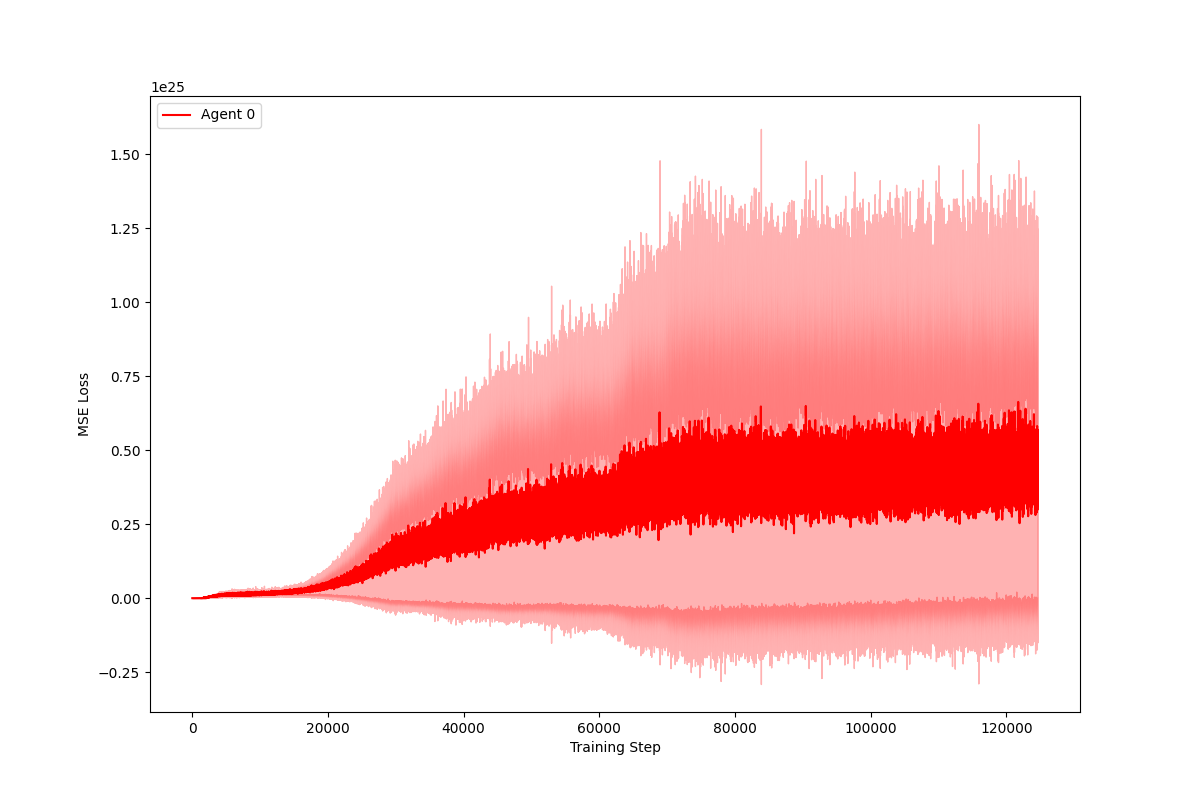
\includegraphics[width=0.55\linewidth]{../../runs/#1/training_losses.png} }
\hfill
\subfloat[Agent Performance\label{fig:#3Returns}]{ 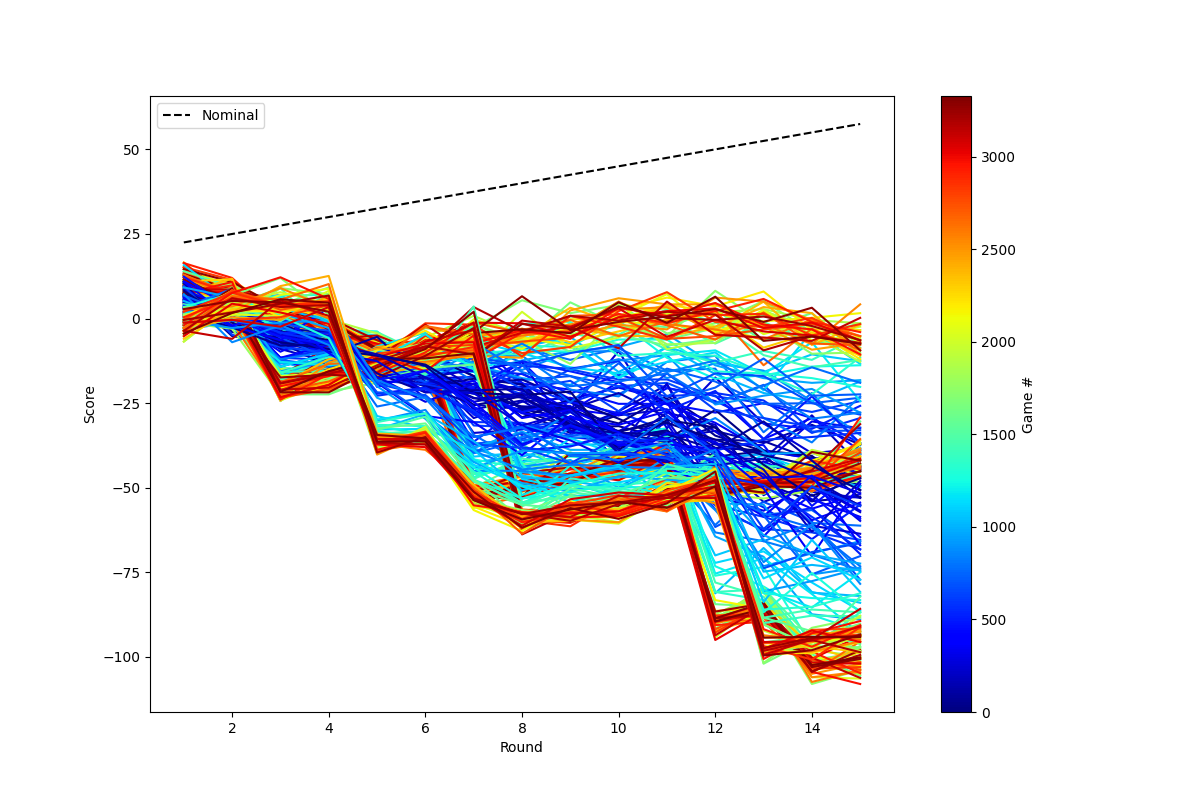
\includegraphics[width=0.6\linewidth]{../../runs/#1/training_returns.png} }
\caption{#2} \label{fig:#3}
\end{figure}
}

Agent performance (Figure \ref{fig:baselineReturns}) was significantly better than random but below human performance. Play proceeds from left to right; older games are shown in blue and newer games in red. Each line is an average of 50 games because there is variation in game to game performance. 'Nominal' performance is marked above, which assumes each agent bets correctly on winning an even share of the available tricks. Initial performance, the dark blue line, is equivalent to random. Since there are more available tricks in later hands, the agent can bet higher, and is likely to lose more points on average. By the end of the training the agent has improved across all rounds except the first but is still on average negative. Figure \ref{fig:human} shows the performance of three of these agents against a human (Agent 0) over five games. These games were shortened to 6 rounds for time. The human performs above the agents but is not out of family.

The reason for these below-nominal results may be seen in the training loss (Figure \ref{fig:baselineLosses}). Loss over time is quite low with occasional spikes. These spikes do not correspond to sudden changes in $\varepsilon$ as one might expect. Rather, some inspection of the data implies that they are the effect of bet information propagating through the system. Betting actions are rare but also very important because an unrealistic bet will make losing points inevitable. So when information about a reward (at the end of a hand) propagates through the $Q(s,a)$ evaluation to the betting action (at the beginning of a hand) it can cause a large shift. The agent has learned not to bet extremely high, which reduces its loss of points later in the game. But it is not accurate enough to bet exactly correct, so it will still lose points in the midgame, but it will lose fewer.

\plotrun{hybrid_2x15_2x5x5_2x16_2x64_pooled}{Baseline Agent}{baseline}

\begin{figure}[h!]
\centering
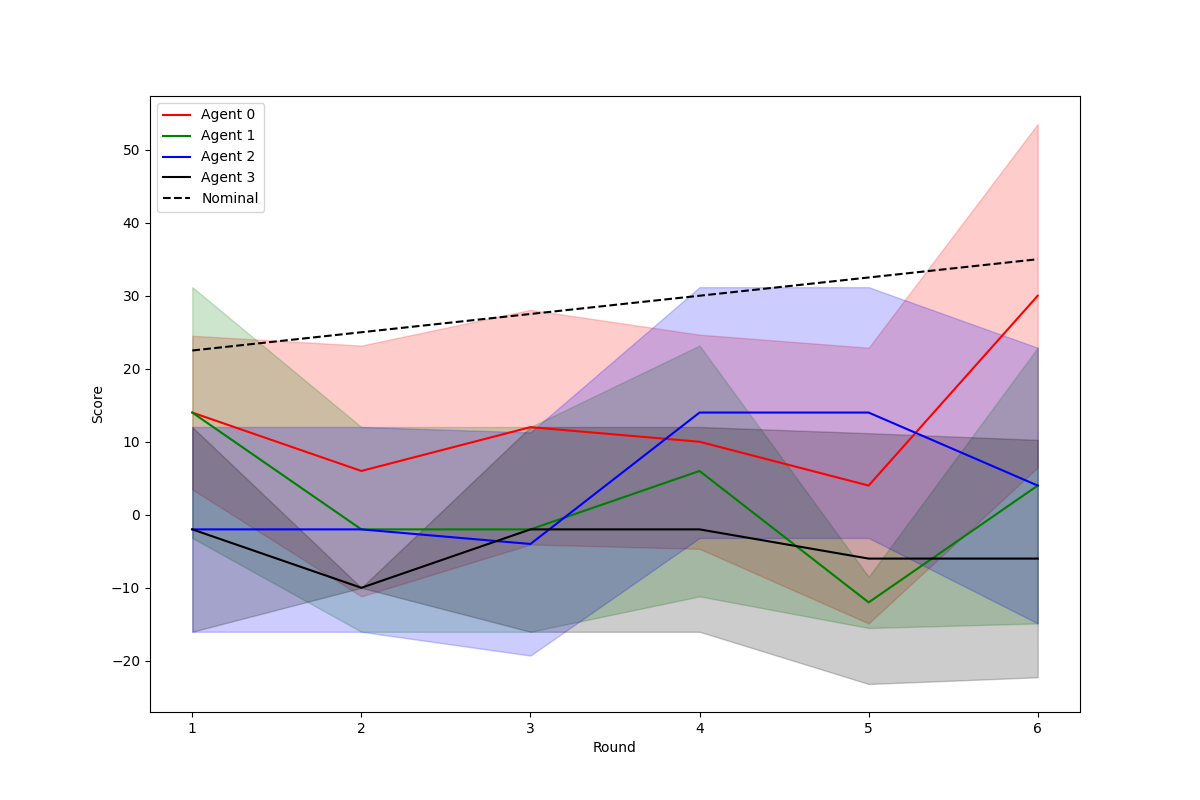
\includegraphics[width=0.55\linewidth]{human_game.png}
\caption{Performance Against Human (Agent 0)} \label{fig:human}
\end{figure}

\newpage

\section{Ablation Study}

In addition to the parameters discussed below, neural net size and epsilon schedule were varied but were not found to have an important effect on agent performance.

\subsection{Buffer Priority}

With rare betting actions very important to gaining points, it makes sense to prioritize them in the replay buffer. A game of $m$ rounds will have $\frac{1}{2}m(m+1)$ playing actions and $m$ betting actions. By increasing the likelihood of selecting a betting action when constructing a training minibatch it should be possible to more closely train these actions. Three strategies were tried for this. Weighting purely by which action was taken, with weights ranging from $[2,10]$, is a simple strategy and can be computed at roughly the same speed as the baseline batch selection, but is chosen arbitrarily. Weighting by the difference between behavior and target value networks, with some floor $\epsilon$ and some exponent $p$, runs at half the speed but should prioritize large updates. Adding a further exponent $\beta$ with its own schedule that will prioritize large updates even more in the early training is slightly slower than that, and also adds another set of hyperparameters that must be tuned.

\begin{table}[h!]
\centering
\begin{tabular}{r|l}
Action-Based & $w = \begin{cases}
2 + \frac{2}{5}m & \text{betting m} \\
1
\end{cases}$ \\
Q-Based & $w = \left( \left|Q_{behavior}(s,a) - Q_{target}(s,a)\right| + \epsilon \right)^p $ \\
Q-Based with Beta Schedule & $w = \left( \left|Q_{behavior}(s,a) - Q_{target}(s,a)\right| + \epsilon \right)^{p\beta}$
\end{tabular}
\end{table}

Action weighting creates a much more consistent loss curve (Figure \ref{fig:aPriorityLosses}) which means the agent is updating more often, but it produces less consistent and often worse scoring (Figure \ref{fig:aPriorityReturns}). The agent seems to be updating its estimations of betting actions more often but it does not understand how to play to its bets. The Q weighting shows a large spike in losses (Figure \ref{fig:qPriorityLosses}) around when the $\varepsilon$ schedule is reaching its minimum, and has similarly inconsistent performance (Figure \ref{fig:qPriorityReturns}). The introduction of a $\beta$ schedule (Figure \ref{fig:qBetaPriorityLosses}) moves the spike earlier as expected but does not fix the scoring (Figure \ref{fig:qBetaPriorityReturns}). Note that a single training session is shown in these plots but results were similar across sessions. Both Q weightings seem to be able to improve on later round performance, and may benefit from very long training sessions, but had very low losses later in training and did not seem to still be learn quickly. The increased runtime of these sessions made investigating this infeasible but it seems promising.

\plotrun{hybrid_2x15_2x5x5_2x16_2x64_pooled_priority}{Action-Based Priority Agent}{aPriority}
\plotrun{hybrid_2x15_2x5x5_2x16_2x64_pooled_q_priority}{Q-Based Priority Agent}{qPriority}
\plotrun{hybrid_2x15_2x5x5_2x16_2x64_pooled_q_beta_priority}{Q-Based Priority Agent with Beta Schedule}{qBetaPriority}

\newpage

\subsection{Agent Pooling}

During training, all four agents were replaced with passthrough agents that fed their experiences into a single buffer and all shared a single neural network. This decreased training time since the pooled agent was learning four times as fast, but raised the possibility of agents being able to predict each others' moves. However, training multiple agents instead of one did not produce significantly different results from the baseline (Figure \ref{fig:unpooled}). Having partial state information was sufficient to make agent actions unpredictable, and the agents also did not converge on a cooperative strategy. If they reached a much higher level of performance, these things might become a concern, and it could be necessary to split them apart. However, it may be possible to do this after they have already reached a base level of competence.

\plotrun{hybrid_2x15_2x5x5_2x16_2x64_unpooled}{Unpooled Agents}{unpooled}

\subsection{Training Algorithm}

In Deep Q Networks, the target network can be evaluated with its own values, or it can be evaluated by instead optimizing expected performance from the current behavior network; this should make the training more stable. However, it did not seem to have an effect in this case (Figure \ref{fig:ddqn}). This is probably due to the fact that the agent was not able to access the information it required in the first place, and that was the reason it could not bet accurately, not that its learning was unstable.

\plotrun{DDQN_hybrid_2x15_2x5x5_2x16_2x64_pooled}{DDQN Agent}{ddqn}

\subsection{Neural Net Architecture}

A very basic neural network composed of two hidden fully connected layers of 64 neurons was the initial architecture. For most 1D state vectors, a convolutional network is not necessary, especially if there are no localizable features. Losses (Figure \ref{fig:fcLosses}) were much higher than for the final agent, and its performance (Figure \ref{fig:fcReturns}) was somewhat better in later hands. However, its performance was very inconsistent, even between training sessions. Presumably without the convolutional encoding of the state the agent was overfitting to its experiences.

\plotrun{DQN_2x64_500k_pooled}{Simple Fully Connected Agent}{fc}

\section{Future Work}

It is apparent that for the attempted agent designs there was either not enough emphasis placed on the betting actions or the agent's learning was not able to effectively take advantage of knowledge about the betting actions. The final architecture was chosen on the assumption that the deck state could be convolved, and this mostly seems to be carried out in the data. Playing and betting actions were kept in the same neural net on the assumption that whatever encoding of the state occurred would be useful for both decisions. However, it might be advantageous to split these phases of play into separate agents. This way, one agent could focus on evaluating the hand and making the bet, and another could focus on playing the hand. This is conceptually similar to the actor-critic method of estimating the value function while also optimizing to it. This would also require training two agents, and may be quite slow. But it would allow for continuing to explore betting actions while exploiting playing actions.

\section{Conclusion}

Agent performance in this environment was middling. The agent was able to improve its performance to a point but not able to replicate human performance. The complex interactions of multiple agents, the large number of state spaces, the large number of actions, and the importance of rare actions do not play to the strengths of simple Deep Q Network agents. More complicated architecture was only able to improve this to a point. With each training run of the baseline agent taking at least 20 minutes on a midline CPU, longer training was not always feasible, but it may also have been necessary. The most promising changes were to the buffer prioritization. Performance was largely unaffected by other minor changes.

\newpage

\begin{algorithm}	
\caption{One Game of Wizard with N Players}\label{alg:game}
\begin{algorithmic}
\Require $3 \leq N \leq 6$
\State choose dealer arbitrarily
\For{hand $M = 1...60/N$} \Comment{each hand can be played independently}
	\State deal each player $M$ cards
	\State flip top card of deck
	\If{top card == wizard} \Comment{rare action benefitting dealer}
		\State dealer chooses trump suit
	\ElsIf{top card == jester \textbf{or} no remaining deck} \Comment{last round always has no trump}
		\State trump suit $\gets$ none
	\Else
		\State trump suit $\gets$ flipped card suit
	\EndIf
	\For{player left of dealer, proceeding left} \Comment{dealer has advantage betting last}
		\State player bets $[1...M]$
	\EndFor
	\State trick leader $\gets$ player left of dealer
	\For{trick $1...M$}
		\State led suit $\gets$ none
		\For{trick leader proceeding left} \Comment{leader has advantage setting suit}
			\If{led suit == none \textbf{or} player does not have led suit}
				\State player plays any card
			\Else
				\State player plays card from led suit \textbf{or} wizard \textbf{or} jester
			\EndIf
			\If{card == wizard}
				\State led suit $\gets$ none for remainder of trick
			\ElsIf{card != jester}
				\State led suit $\gets$ played suit
			\EndIf
		\EndFor
		\State winner leads next trick
	\EndFor
	\For{player $1...N$}
		\If{won tricks == bet tricks} \Comment{betting correctly is highly rewarding}
			\State points $+= 20 + won \cdot 10$
		\Else
			\State points $-= 10 \cdot |won - bet|$
		\EndIf
	\EndFor
	\State dealer proceeds left
\EndFor
\end{algorithmic}
\end{algorithm}

\end{document}
